\section{Introduction}
\label{sec:intro}


In these laboratory assignement the objective is to use an AC/DC converter to obtain a DC signal as an output. The DC signal must be a value of 12V from an AC signal with an amplitude of 230V and a frequency of 50Hz. The envelope detector and voltage regulator circuits were chosen by us as shown in Figure.


\begin{figure} [!htb] 
  \minipage{0.9\textwidth}
  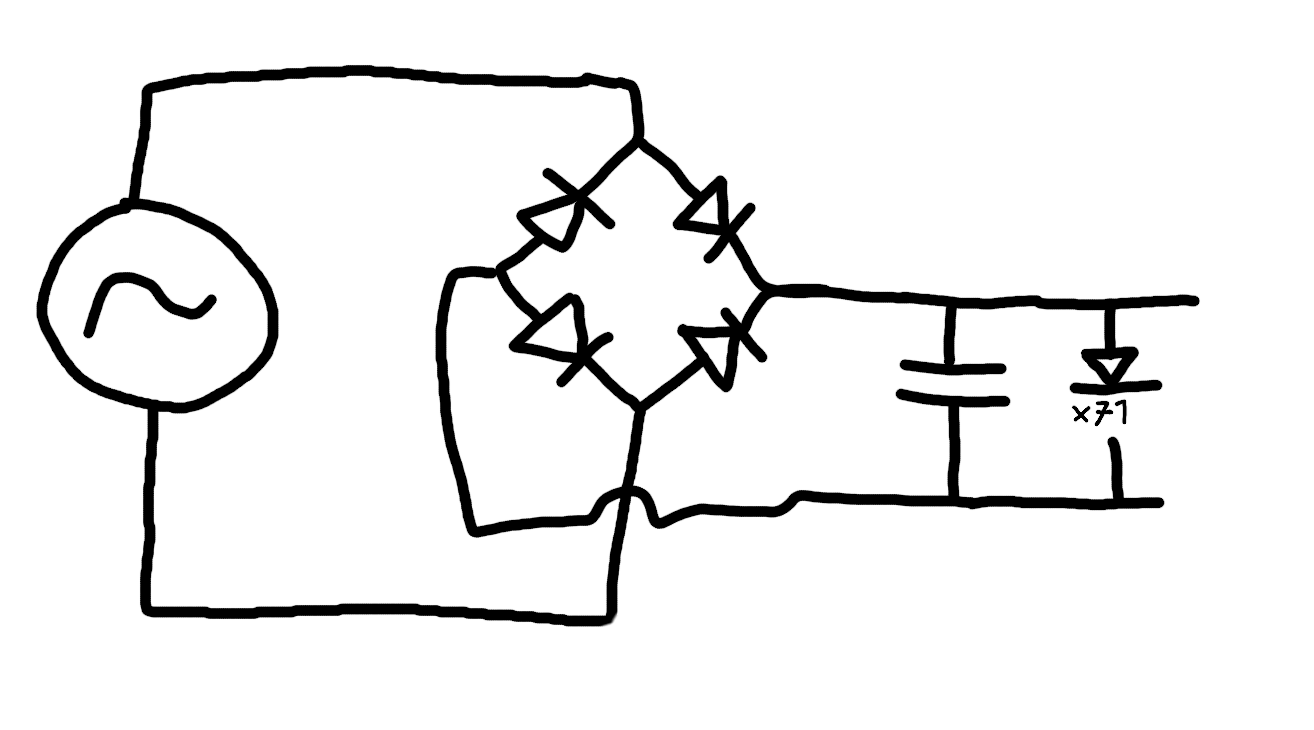
\includegraphics[width=\linewidth]{circuito.png}
  \caption{Circuit used in this laboratory}
  \label{fig:theoplots}
  \endminipage\hfill
\end{figure}

This peculiar design was chosen because of the specifications of the prompt for this assignment. The circuit presented makes use of a single small capacitor and a large stack of diodes in series. This does not make it a useful power supply, but it fits within the requirements of the assignment, and produces a steady 12V supply with minimal cost compared to other solutions. This works by stripping a normal envelope detector and limiter circuit of its resistors, and using an oversized limiter as the discharge resistor for the capacitor, behaving as a several megaohm resistor instead of voltage limiter.
